\chapter{Appendix A - Concept Map}
\label{appendix:A}
% concept map

\begin{figure}[h!]
\centering
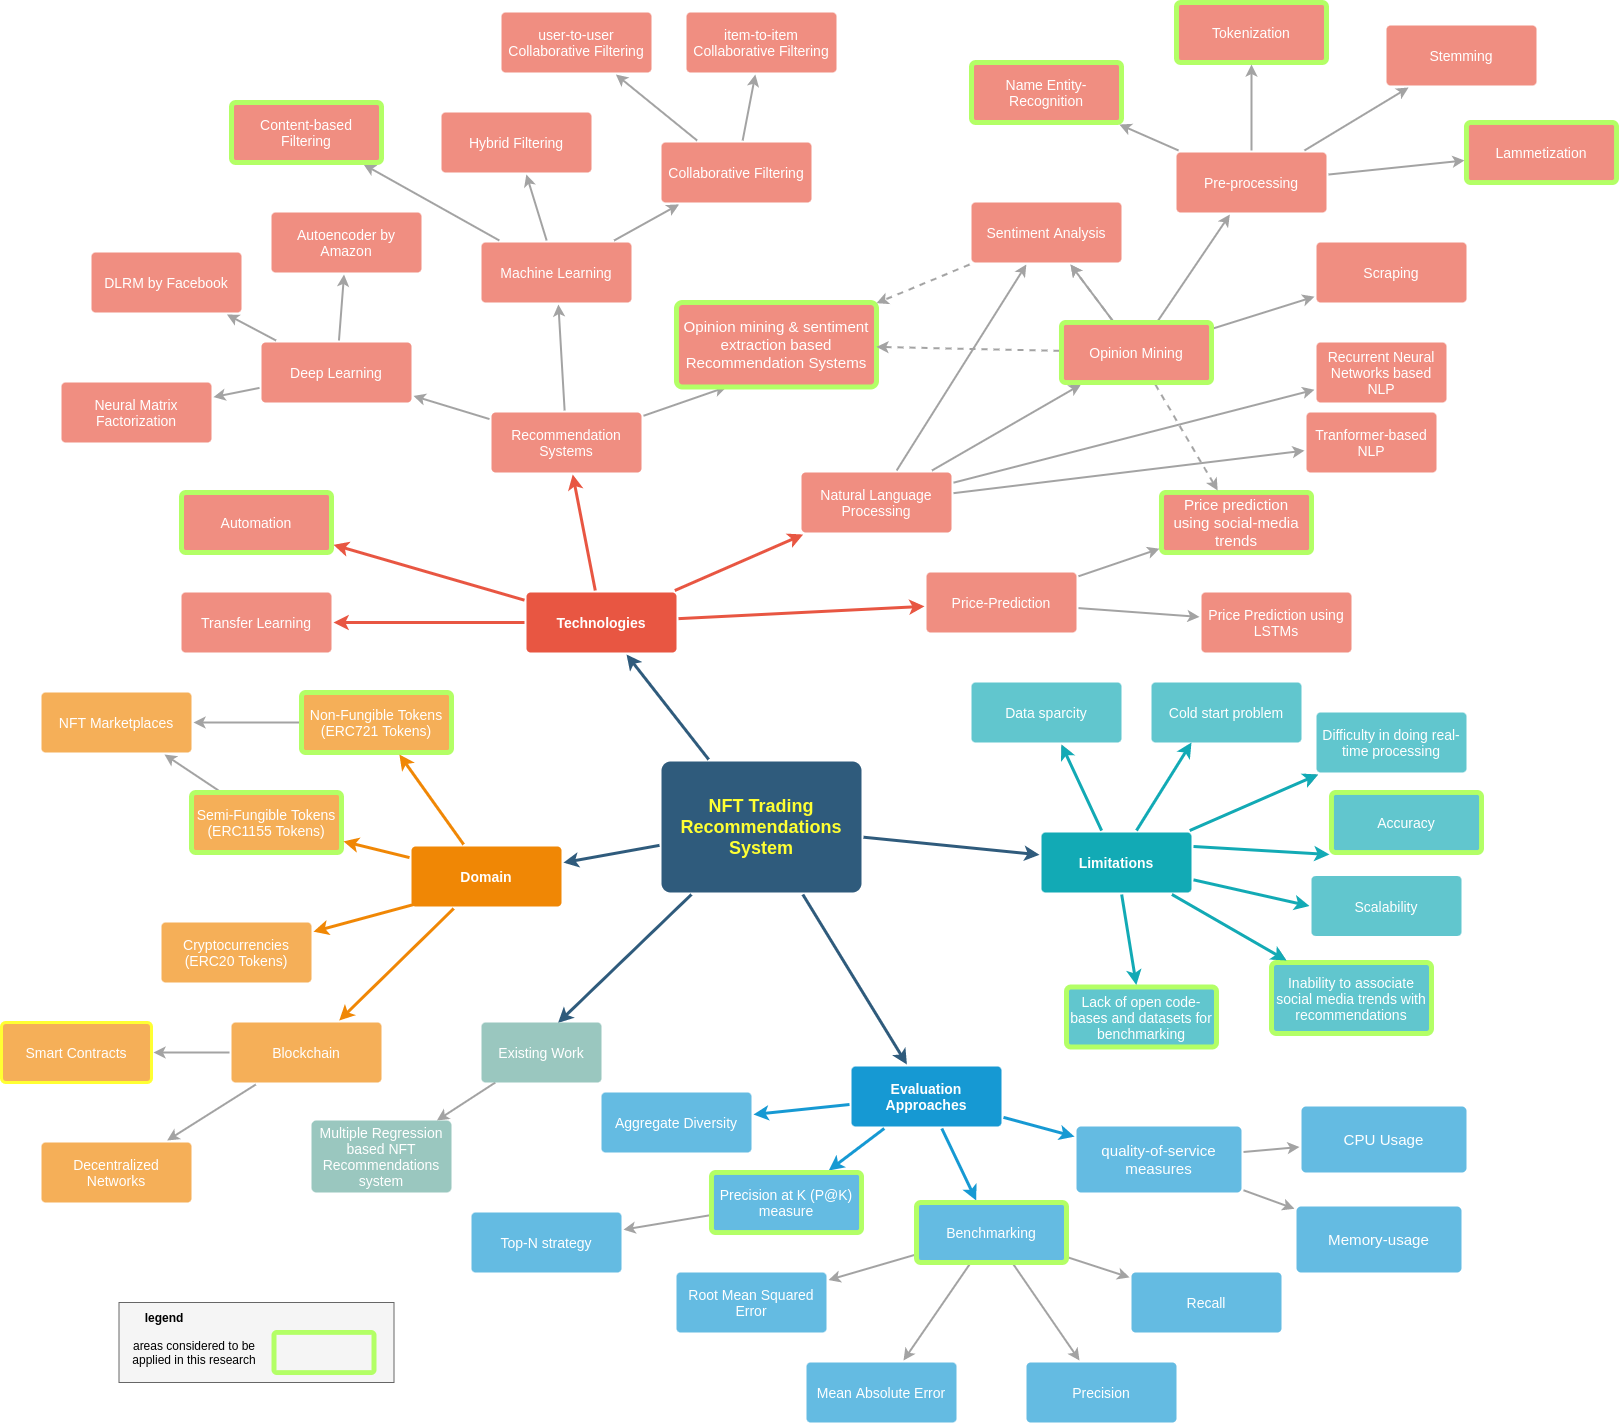
\includegraphics[width=\textwidth]{images/appendix/concept-map.png}
\caption{Concept Map \textit{(self-composed)}}
\label{fig:concept-map}
\end{figure}

% \chapter{Appendix B - Work Breakdown Structure}

% \chapter{Appendix  - Requirement Engineering Survey}


\chapter{Appendix C - Evaluations}
\label{appendix:C}

\section*{Appendix C1 - Evaluations received by Evaluators}

% TODO: have a table for each cateogry/ separate by category row.

\begin{longtable}{|p{0.17\linewidth}|p{0.17\linewidth}|p{0.56\linewidth}|}
\caption{Evaluations received by Evaluators}
\label{tab:evaluators-eval-feedback}
\\
\hline
\textbf{Evaluator} & \textbf{Qualifications/ Position of Employment} & \textbf{Feedback} \endfirsthead
\hline
 &  &  \\
\hline
 &  &  \\
\hline
 &  &  \\
\hline
 &  & \\
\hline
\end{longtable}


\section*{Appendix C2 - Evaluation of Functional Requirements}

\vspace{-4mm}
\begin{longtable}{|l|p{0.5\linewidth}|c|l|l|}
\caption{Evaluation of the implementation of Functional Requirements}
\label{tab:eval-func-requirements}
\\ 
\hline
\begin{tabular}[c]{@{}l@{}}\textbf{FR}\\\textbf{ID}\end{tabular}
& \textbf{Requirement} & \begin{tabular}[c]{@{}c@{}}\textbf{Priority}\\\textbf{Level}\end{tabular} & 
\begin{tabular}[c]{@{}c@{}}\textbf{Use}\\\textbf{Case}\end{tabular} & \textbf{Evaluation}
\endfirsthead 
\hline
FR1 & Users must be able to add a chosen NFT to be considered as the reference point to generating recommendations. & M & UC1 & \\ 
\hline
FR2 & Admins should be able to add a collection of NFT to be used as recommendations. & S & UC1 & \\ 
\hline
FR3 & The system could be able to fetch relevant data of the NFT using an entered token Id. & C & UC1 & \\ 
\hline
FR4 & Users must be able to set/ adjust the bias and parameters to be used by the Recommendations System using parametric selections prior to generating recommendations. & M & UC2 & \\ 
\hline
FR5 & Admins should be able to adjust the default bias of the Recommendations System. & S & UC3 & \\ 
\hline
FR6 & Users must be able to view recommendations with the click of a button. & M & UC4 & \\
\hline
FR7 & The prototype could have an option to receive user feedback regarding the satisfaction level of the generated recommendations by the system. & C & UC4 & \\
\hline
FR8 & The system could show the reasons for recommending each item to users. & C & UC4 & Implemented \\
\hline
FR9 & The system should generate price predictions and consider the results for recommendations. & S & UC5 & \\ 
\hline
FR10 & Opinion mining trends data must be used to generate \gls{nft} recommendations. & M & UC7 & Implemented \\
\hline
FR11 & A user could be allowed to feed data-points such as interested public figures, websites to use as opinion mining data for recommendations. & C & UC8 & \\ 
\hline
FR12 & Admins should be able to~feed data-points such as interested public figures, websites to use as opinion mining data for recommendations. & S & UC8 & \\
\hline
FR13 & User-input could be aggregated and used as a reinforcement learning bias for the Recommendations Model. & C & &  \\
\hline
FR14 & The system will not act as a decentralized system. & W & &  \\
\hline
% FR15 search NFTs by tags?
\multicolumn{5}{|c|}{
Functional Requirement Completion Percentage = $\frac{}{14} * 100$ = \%
}\\
\hline
\end{longtable}


\section*{Appendix C3 - Evaluation of Non-Functional Requirements}

\vspace{-4mm}
\begin{longtable}{|l|l|l|l|}
\caption{Evaluation of the implementation of Non-functional requirements}
\label{tab:eval-non-func-requirements}
\\ 
\hline
\textbf{NFR ID} & \textbf{Requirement} & \textbf{Priority Level} &  \textbf{Evaluation} \endfirsthead 
\hline
1 & Performance & Desirable & Implemented \\ 
\hline
2 & Quality of Output & Important & Implemented \\ 
\hline
3 & Security & Desirable & \\ 
\hline
4 & Usability & Important & \\ 
\hline
5 & Scalability & Desirable & \\
\hline
\multicolumn{4}{|c|}{
Non-Functional Requirement Completion Percentage = $\frac{}{5} * 100$ = \%
}\\
\hline
\end{longtable}